\newpage
\section{Skinning}

\begin{figure}[!htb]
    \centering
    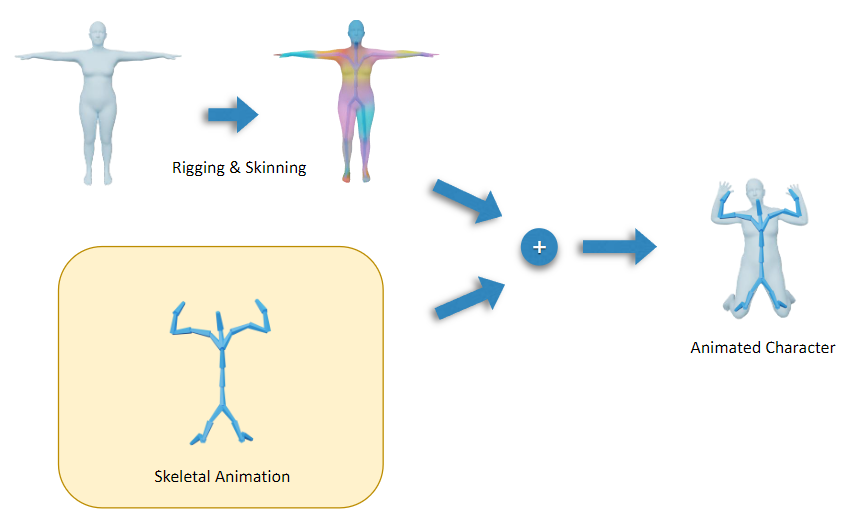
\includegraphics[width=0.618\linewidth]{pic/1057/Character Animation Pipeline}
    \caption{Character Animation Pipeline}
\end{figure}


\begin{itemize}
    \item Rigging: 绑定, 可能会添加额外控制器.
    \item Skinning: 特殊的绑定, 将皮肤绑定到骨骼.
\end{itemize}

Skinning Deformation: 
\begin{align*}
    \bx' &= Q'Q^\top (\bx - \bo) + \bo'\\
    &= Q' \br + \bo'\\
    Q' &= RQ\\
    \bo' &= \bo + \bt\\
    \br &= Q^\top (\bx - \bo)
\end{align*}
$\br$ 表示关节到蒙皮的局部坐标. 

\begin{figure}[!htb]
    \centering
    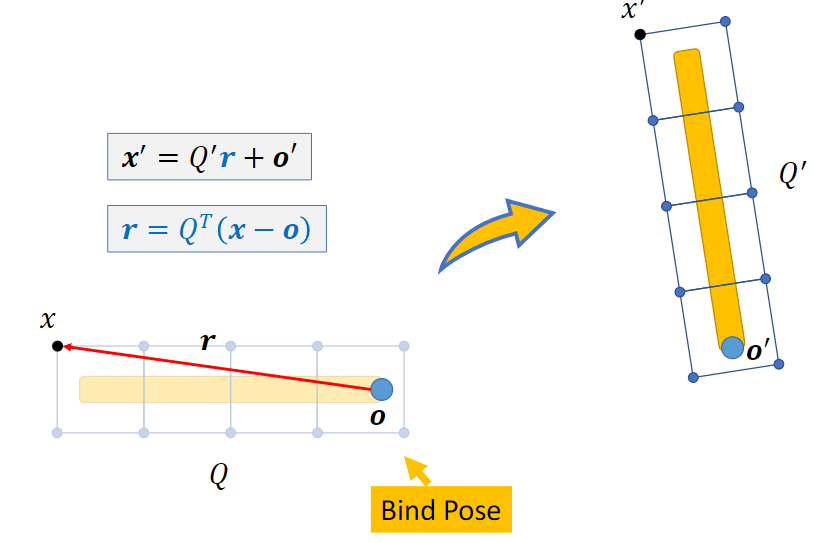
\includegraphics[width=0.618\linewidth]{pic/1057/Skinning Deformation}
    \caption{Skinning Deformation}
\end{figure}

Bind Pose: 在此姿态下计算 $\br$

对于多个骨骼, 在没旋转之前
\begin{align*}
    \br_1&= Q_1^\top (\bx-\bo_1)\\
    \br_2&=Q_2^\top (\bx-\bo_2)
\end{align*}
在旋转之后
\begin{align*}
    \bx'_1&=Q_1'\br_1 + \bo_1'\\
    \bx'_2&=Q_2'\br_2 + \bo_2'\\
    \bx' &= w_1\bx_1'+w_2\bx_2'
\end{align*}
但是旋转后一个点变成了两个点, 所以加个权重混合这两个点.

\begin{figure}[!htb]
    \centering
    \begin{subfigure}{0.618\linewidth}
        \centering
        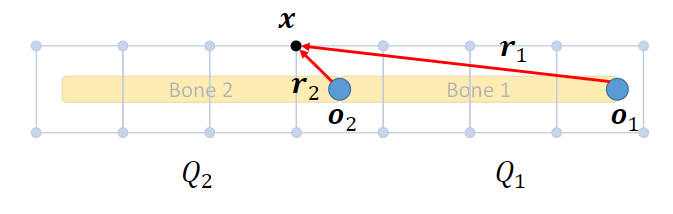
\includegraphics[width=\linewidth]{pic/1057/Skinning Deformation1}
        % \caption{Skinning Deformation1}
    \end{subfigure}
    \begin{subfigure}{0.618\linewidth}
        \centering
        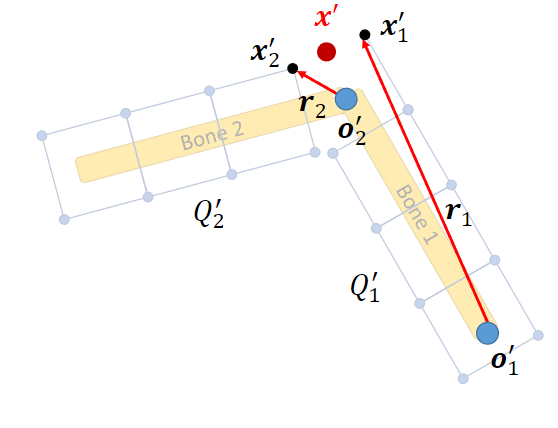
\includegraphics[width=\linewidth]{pic/1057/Skinning Deformation2}
        % \caption{}
    \end{subfigure}
    \caption{Skinning Deformation}
\end{figure}


\subsection{Linear Blend Skinning (LBS)}
线性混合蒙皮.
\begin{figure}[!htb]
    \centering
    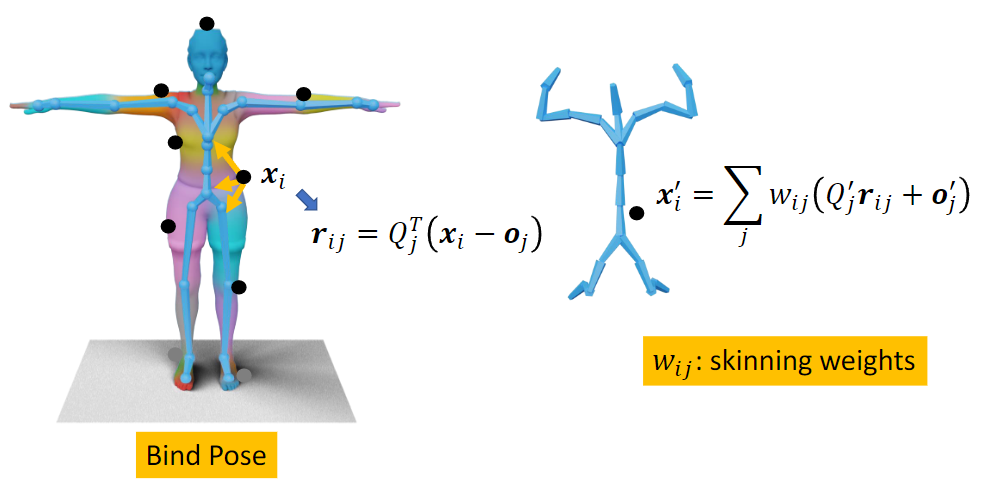
\includegraphics[width=0.88\linewidth]{pic/1057/Skinning}
    \caption{Skinning}
\end{figure}

\begin{itemize}
    \item 在 Bind pose / rest pose: 和 t-pose 不同, 其局部旋转不一定为 0
    \item 用 Skinning weights: 决定蒙皮质量
    \item 得到 Skinning transformation
\end{itemize}
这种方法高效, 且可并行, 游戏很常用. 

\begin{align*}
    \bx_i'&=\sum_{j=1}^m w_{ij}(Q_j'\br_{ij}+\bo_j')\\
    &=\sum_{j=1}^m w_{ij} \left(Q_j'Q_j^\top (\bx_i - \bo_j)+\bo_j'\right)\\
    &=\sum_{j=1}^m w_{ij} \left(Q_j'Q_j^\top \bx_i + \left(\bo_j' - Q_j'Q_j^\top  \bo_j \right)\right)\\
    &=\sum_{j=1}^m w_{ij}\left(R_j \bx_i + \bt_j\right)
\end{align*}

\begin{align*}
    \bx_i'&=\sum_{j=1}^m w_{ij}(R_j \bx_i + \bt_j)\\
    &=\sum_{j=1}^m w_{ij} R_j \bx_i + \sum_{j=1}^m w_{ij}\bt_j\\
    &=\left(\sum_{j=1}^m w_{ij} R_j \right)\bx_i + \sum_{j=1}^m w_{ij}\bt_j
\end{align*}



但是 $\left(\sum_{j=1}^m w_{ij} R_j \right)$ 是旋转矩阵的线性插值, 很容易出现插值后结果非线性矩阵的问题. 这种现象叫做 Candy-Wrapper Artifact (糖纸效应)

也不能换用其他可以插值的旋转表示, 因为其他旋转表示相对的是原点, 如果插值其和位移的配合是不好的.


\subsection{Dual Quaternion Skinning (DQS)}
用非线性变换来解决. 
%TODO 摸了, 后面记得来补. P43, 43:15
% 逆天, 补一下李代数和李群吧 https://zhuanlan.zhihu.com/p/358455662


\subsection{Blendshapes}

\subsection{Examples}

\subsubsection{The SMPL model}

\subsubsection{Facial Animation}